% Print slides
% backup report and presentation (github)
% Enjoy 
\documentclass[10pt]{beamer}

\usetheme[progressbar=frametitle]{metropolis}
\usepackage{appendixnumberbeamer}

\usepackage{booktabs}
\usepackage[scale=2]{ccicons}
\usepackage{dirtytalk} % \say{inline quote}
\usepackage{csquotes} % \begin{displayquote} larger quote \end{displayquote}
\usepackage{natbib}
\usepackage[Algoritm]{algorithm}
\usepackage{algpseudocode}
\usepackage{caption}
\usepackage{amsmath}
\usepackage{amssymb}
\usepackage{amsthm}

\usepackage{pgfplots}
\usepgfplotslibrary{dateplot}

\usepackage{xspace}
\newcommand{\themename}{\textbf{\textsc{metropolis}}\xspace}

\title{An Impact Measurement Manager Approach to AI Safety}
\subtitle{Master's thesis in Mathematical Statistics, Statistical Learning and AI}
% \date{\today}
\date{2022 - 12th of October}
\author{Jonatan Hellgren}
\institute{Department of Mathematical Sciences\\
Chalmers University of Technology\\
University of Gothenburg}
% \titlegraphic{\hfill\includegraphics[height=1.5cm]{logo.pdf}}

\begin{document}

\maketitle

\begin{frame}
  \begin{tabular}[t]{lll}
  Supervisor:& Olle Häggström, Department of Mathematical Sciences,\\
    & Chalmers University of Technology\\
  Examiner:& Torbjörn Lundh, Department of Mathematical Sciences,\\
    & Chalmers University of Technology\\
  Opponents:& Jens Ifver and Calvin Smith\\ & Universty of Gothenburg
  \end{tabular}
\end{frame}

% \begin{frame}{Table of contents}
  % \setbeamertemplate{section in toc}[sections numbered]
  % \tableofcontents%[hideallsubsections]
% \end{frame}

\section{Introduction}

\begin{frame}{Aim of Thesis}
  \begin{columns}[T,onlytextwidth]

    \column{0.5\textwidth}
      \Large{Investigation}

      \large
      \begin{itemize}[<+- | alert@+>]
        \item Provide an in-depth investigation on current litterature on AI safety.
        \item Specifically, low-impact AIs using impact measurements.
      \end{itemize}

    \column{0.5\textwidth}
      \Large{Simulation}

      \large
      \begin{itemize}[<+- | alert@+>]
        \item Propose a novel impact measurement.
        \item Evaluate it in different environmets.
        \item Compare the results with the current litterature.
      \end{itemize}

  \end{columns}
\end{frame}

\begin{frame}{Overview of Presentation}
  % We will begin with a description of the title
  \begin{itemize}[<+- | alert@+>]
    \item We will begin by looking at \textbf{AI safety}.
    \item Then go on with \textbf{impact measurements}.
    \item After that, I will explain the \textbf{manager approach}.
    \item Finally, I will present the results.
  \end{itemize}
  % Then move on to the results, discussion, and conclusion
\end{frame}

% \begin{frame}{Overview of Presentation}
  % We will begin with a description of the title
  % \begin{itemize}
    % \item AI safety
    % \item Impact measurement
    % \item Manager approach
  % \end{itemize}
% \end{frame}

\section{AI Safety}

\begin{frame}{Why should we worry?}
  \begin{itemize}[<+- | alert@+>]
    \item What is Artificial Intelligence (AI)?
    \item AI will likely become more intelligent then us.
    \item The strength of Homo Sapiens - intelligence.
    % \item 
  \end{itemize}
   
\end{frame}

\begin{frame}{Risk of existential catastrophe}
  \begin{columns}[T,onlytextwidth]

    \column{0.5\textwidth}
    Toby Ord in his book \textit{The Precipice} loosely estimates the chance of a existential catastrophe in the upcoming century to be: \visible<2->{1 in 6, out of which 1 in 10 is due to unaligned AI, see \citet{Precipice}} \\
    \column{0.5\textwidth}
    \centering
  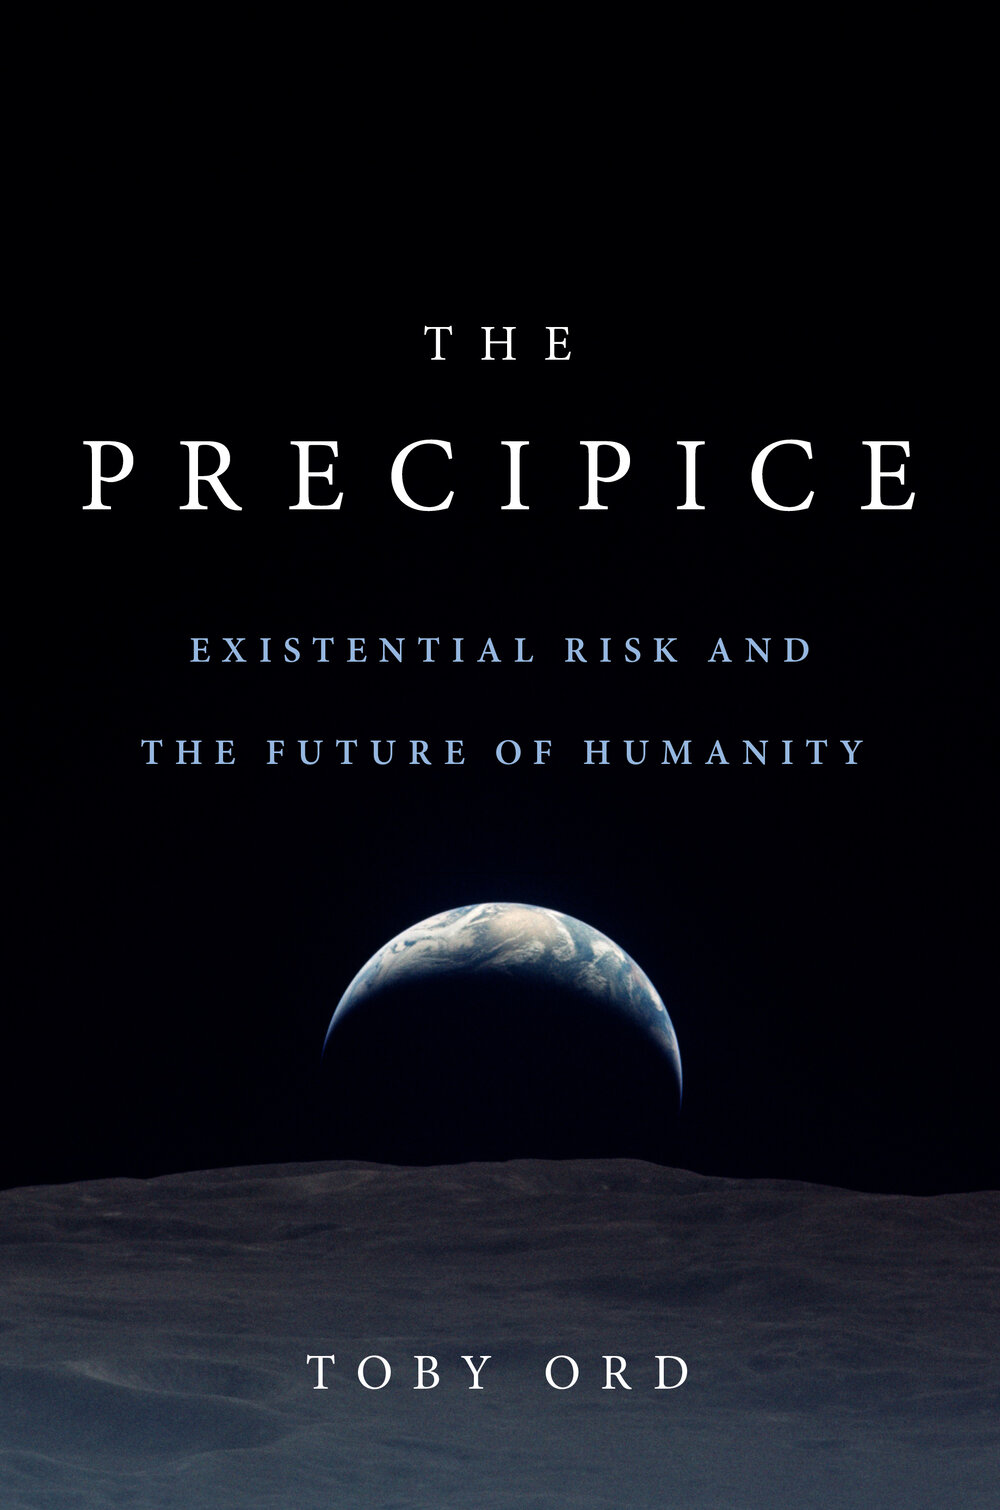
\includegraphics[scale=0.4]{images/precipice.jpg}
  \end{columns}
\end{frame}

\begin{frame}{Future progress}
  To differentiate current AI from future versions, several terms are used:
  \begin{itemize}
    \visible<2->{\item Artificial General Intelligence (AGI):
      \begin{displayquote}
        An AI that can solve an arbitrary set of tasks with\\ as good or better performance then a human. 
      \end{displayquote}}
      % In other words: Can pick up any task and solve it without any human intervention how it should be done.
      % Connect back to humans intelligence has been the driving force for innovation. Now when this is being automated. Impacts of AGI will be likely on the same scale as the industial revolution
    \visible<3->{\item Transformative AI (TAI):
      \begin{displayquote}
      An AI system capable enough to induce transformative\\ consequences on the same scale as the industrial or\\ agricultural revolution.
      \end{displayquote}}
      % Example of how this can happen. Convincing speech bot.
    \visible<4->{\item Prepotent AI:
      \begin{displayquote}
        An TAI that once deployed would be unstoppable.
      \end{displayquote}}
  \end{itemize}
\end{frame}

\begin{frame}{Existential risk}

  \begin{columns}[T,onlytextwidth]

    \column{0.5\textwidth}
    On futureoflife.org we find the following description, see \citet{FLI}:\\

    \visible<2->{
      An existential risk is any risk that has the potential to eliminate all of humanity or, at the very least, kill large swaths of the global population, leaving the survivors without sufficient means to rebuild society to current standards of living.}
    \column{0.4\textwidth}
  
\includegraphics[scale=0.1]{images/FLI.png}
    % \begin{itemize}
      % \item Future of Life (FLI) is an independent non-profit,
      % \item reduce extreme risks from transformative technologies,
      % \item steer the development and use of these technologies to benefit life.
    % \end{itemize}
  \end{columns}
\end{frame}

\begin{frame}{The human fragility argument}
  % A quick description of artificial intelligence, to make sure we are on the same page.
  \begin{columns}[T,onlytextwidth]

    \column{0.5\textwidth}
    In \citet{CritchKruger} we find the human fragility argument.\\
    \textbf{Human fragility argument:}
    \visible<2->{ Most potential future states of the Earth are unsurvivable to humanity.} \visible<3->{Therefore, deploying a prepotent AI system absent any effort to render it safe to humanity is likely to realize a future state which is unsurvivable. }
    \column{0.5\textwidth}
    \centering
  
\includegraphics[scale=0.4]{images/CritchKrueger.png}
    % \begin{itemize}
      % \item Future of Life (FLI) is an independent non-profit,
      % \item reduce extreme risks from transformative technologies,
      % \item steer the development and use of these technologies to benefit life.
    % \end{itemize}
  \end{columns}
\end{frame}


\begin{frame}{Timeline for TAI Breakthrough}
  \begin{itemize}[<+- | alert@+>]
  \item Many predictions for this has been made. 
  \item However, the most extensive work I have seen is made by \citet{Ajeya}, Senior Research Analyst at Open Philanthropy, with her work on forecasting TAI with biological anchors. (over 150 pages) 
  % \item Median 2050 for development of TAI.
  \item 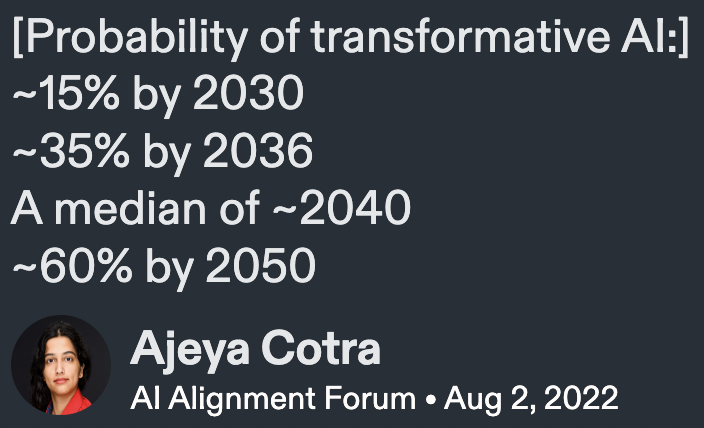
\includegraphics[scale=0.2]{images/prediction.png}
  \end{itemize}

\end{frame}

\begin{frame}{AI Alignment}

  \begin{columns}[T,onlytextwidth]

    \column{0.5\textwidth}
    \textbf{AI alignment:}
    \visible<2->{AI alignment refers to goals of the AI being in line and not conflicting with the intended goal. } \visible<3->{Therefore, an AI that does something at cross-purposes to the intended goal is called unaligned.}
    \column{0.5\textwidth}
    \centering
    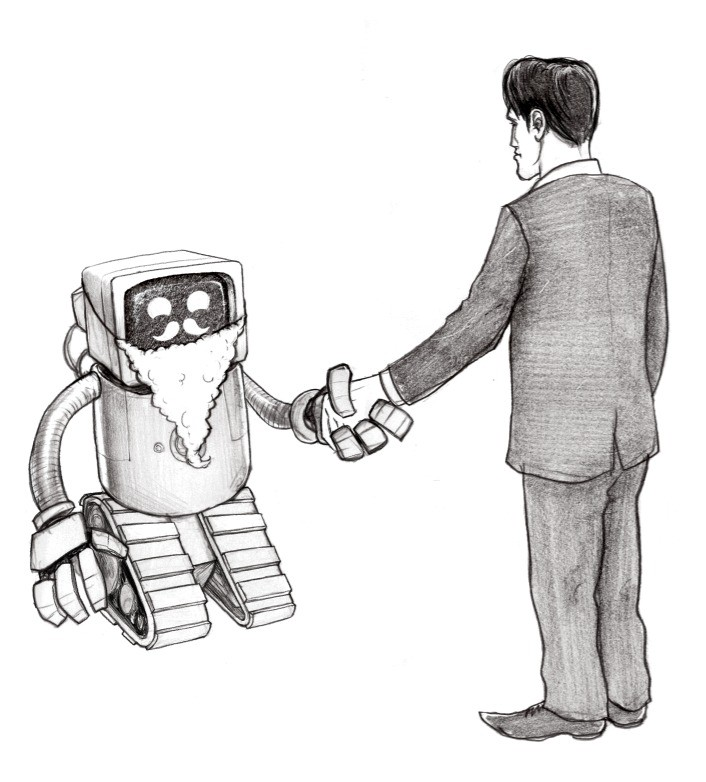
\includegraphics[scale=0.15]{figures/agreeing.jpeg}\\
    \tiny{\textcopyright: Ben Gilburt }
    % \begin{itemize}
      % \item Future of Life (FLI) is an independent non-profit,
      % \item reduce extreme risks from transformative technologies,
      % \item steer the development and use of these technologies to benefit life.
    % \end{itemize}
  \end{columns}
\end{frame}


\section{Approaches for creating safe AI}

\begin{frame}{Approaches for creating safe AI}
  \begin{itemize}[<+- | alert@+>]
      \item There exists several approaches.
      \item For example, corrigibility and interruptibility.
      \item And, inverse reinforcement learning.
      \item But I have focused on side effect minimization.
  \end{itemize}
\end{frame}

\begin{frame}{Side effects}

  \begin{columns}[T,onlytextwidth]

    \column{0.5\textwidth}
    \textbf{Side effect:}\\
    \visible<2->{When an AI impacts the environment in a way that is unnecessary for achieving its objective.}
    \column{0.5\textwidth}
    \centering
    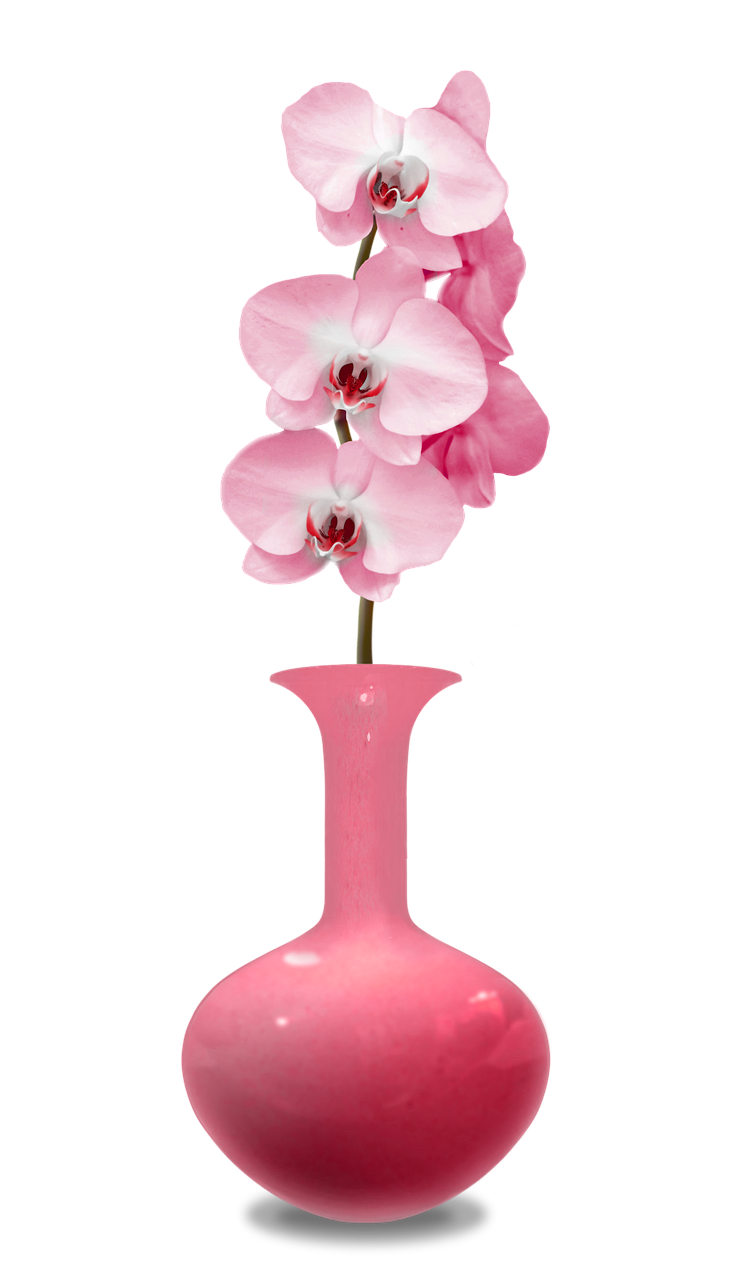
\includegraphics[scale=0.1]{images/vase.png}\\
    % \begin{itemize}
      % \item Future of Life (FLI) is an independent non-profit,
      % \item reduce extreme risks from transformative technologies,
      % \item steer the development and use of these technologies to benefit life.
    % \end{itemize}
  \end{columns}
\end{frame}


\begin{frame}{Low impact AI}
  % First mention that there are several different ways for creating safe AI. 
  \begin{itemize}[<+- | alert@+>]
    \item In \citet{ArmstrongLevinstein} the authors lay the philosophical ground work for low impact AI. 
    \item The idea is to penalize the AI based on its impact.
    \item The key here is to find the right value for the penalization.\\
    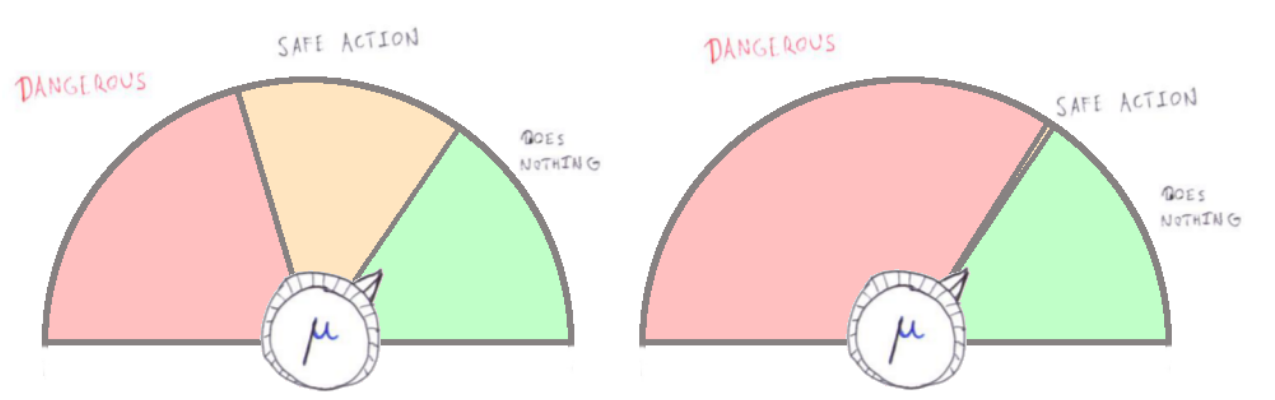
\includegraphics[scale=0.2]{images/dial.png}
  \end{itemize}
  
\end{frame}

\begin{frame}{Impact measurements}
  \begin{itemize}[<+- | alert@+>]
    \item Impact measurements is the low impact AI ideas applied to AI agents. 
    \item An AI agent is an AI that is located and acts in a environment.\\
  % \documentclass{article}
% \usepackage[utf8]{inputenc}
% \usepackage{tikz}
% \begin{document}

\centering
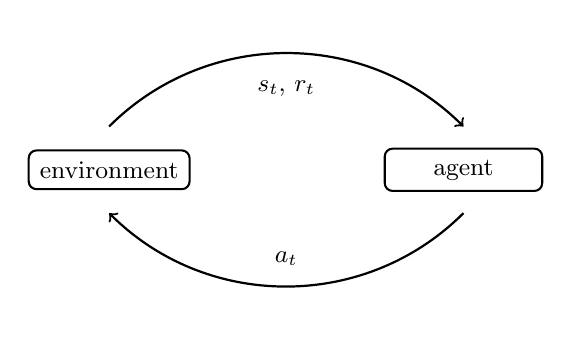
\begin{tikzpicture}[
  % GLOBAL CFG
  % font=\sf \scriptsize,
  % Styles
  cell/.style={% For the main box
      rectangle, 
      rounded corners=5mm, 
      draw,
      very thick,
      },
  operator/.style={%For operators like +  and  x
      circle,
      draw,
      inner sep=-0.5pt,
      minimum height =.4cm,
      },
  function/.style={%For functions
      ellipse,
      draw,
      inner sep=1pt
      },
  ct/.style={% For external inputs and outputs
      rectangle, 
      rounded corners=1mm, 
      draw,
      line width = .75pt,
      minimum width=1cm,
      inner sep=4pt,
      },
  gt/.style={% For internal inputs
      rectangle,
      draw,
      minimum width=10mm,
      minimum height=6mm,
      inner sep=1pt
      },
  empty/.style={% Empty nodes for joining arrows
      rectangle,
      draw,
      minimum width=0mm,
      minimum height=0mm,
      inner sep=0pt
      },
  mylabel/.style={% something new that I have learned
      font=\scriptsize\sffamily
      },
  ArrowC1/.style={% Arrows with rounded corners
      rounded corners=.25cm,
      thick,
      },
  ArrowC2/.style={% Arrows with big rounded corners
      rounded corners=.5cm,
      thick,
      },
  ]
    
    %Start drawing the thing...    

  % Draw the cell: 
  % \node [cell, minimum height =1cm, minimum width=3cm] at (0,0){\small Environment} ;
  % \node [cell, minimum height =1cm, minimum width=3cm] at (4.5,0){\small Agent} ;


  \node [ct, minimum width=2cm] (optim1) at (0,0) {\small environment}; 
  \node [ct, minimum width=2cm] (optim1) at (4.5,0) {\small agent}; 

  \node [empty, label={\small $a_t$}] (action) at (2.25, -1.35) {};
  \node [empty, label={\small $s_t$, $r_t$}] (state) at (2.25, 0.8) {};

  \draw [->, thick] (0, 0.55) to[out=45,in=135] (4.5, 0.55);
  \draw [->, thick] (4.5, -0.55) to[out=-135,in=-45] (0, -0.55);
  


\end{tikzpicture}

% \end{document}

    \item The impact measurement is added to the reward function.
    \[ R^\prime(s_{t}) := R(s_{t}) - \lambda d(s_{t}, s_{t}^\prime). \]
  \end{itemize}

\end{frame}


\section{Manager Approach}

\begin{frame}{Reinforcement learning}
  Reinforcement Learning (RL)
  % \documentclass{article}
% \usepackage[utf8]{inputenc}
% \usepackage{tikz}
% \begin{document}

\centering
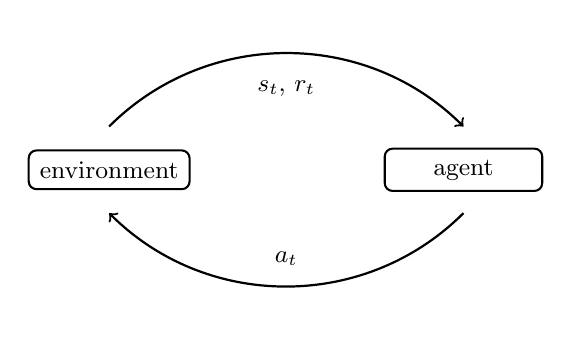
\begin{tikzpicture}[
  % GLOBAL CFG
  % font=\sf \scriptsize,
  % Styles
  cell/.style={% For the main box
      rectangle, 
      rounded corners=5mm, 
      draw,
      very thick,
      },
  operator/.style={%For operators like +  and  x
      circle,
      draw,
      inner sep=-0.5pt,
      minimum height =.4cm,
      },
  function/.style={%For functions
      ellipse,
      draw,
      inner sep=1pt
      },
  ct/.style={% For external inputs and outputs
      rectangle, 
      rounded corners=1mm, 
      draw,
      line width = .75pt,
      minimum width=1cm,
      inner sep=4pt,
      },
  gt/.style={% For internal inputs
      rectangle,
      draw,
      minimum width=10mm,
      minimum height=6mm,
      inner sep=1pt
      },
  empty/.style={% Empty nodes for joining arrows
      rectangle,
      draw,
      minimum width=0mm,
      minimum height=0mm,
      inner sep=0pt
      },
  mylabel/.style={% something new that I have learned
      font=\scriptsize\sffamily
      },
  ArrowC1/.style={% Arrows with rounded corners
      rounded corners=.25cm,
      thick,
      },
  ArrowC2/.style={% Arrows with big rounded corners
      rounded corners=.5cm,
      thick,
      },
  ]
    
    %Start drawing the thing...    

  % Draw the cell: 
  % \node [cell, minimum height =1cm, minimum width=3cm] at (0,0){\small Environment} ;
  % \node [cell, minimum height =1cm, minimum width=3cm] at (4.5,0){\small Agent} ;


  \node [ct, minimum width=2cm] (optim1) at (0,0) {\small environment}; 
  \node [ct, minimum width=2cm] (optim1) at (4.5,0) {\small agent}; 

  \node [empty, label={\small $a_t$}] (action) at (2.25, -1.35) {};
  \node [empty, label={\small $s_t$, $r_t$}] (state) at (2.25, 0.8) {};

  \draw [->, thick] (0, 0.55) to[out=45,in=135] (4.5, 0.55);
  \draw [->, thick] (4.5, -0.55) to[out=-135,in=-45] (0, -0.55);
  


\end{tikzpicture}

% \end{document}

\end{frame}

\begin{frame}{Reinforcement learning}
  \begin{itemize}[<+- | alert@+>]
    \item I will use a variation of Proximal Policy Optimization (PPO), as described in \citet{schulman2017proximal}.
    \item It is a actor-critic method. 
    \item The actor and the critic are both neural networks.
  \end{itemize}
  
  \visible<4->{\[L^{CLIP}(\theta) = \mathbb{E}_t \left [ \min(\delta_t(\theta) \ \hat{A}_t,\ 
\text{clip}(\delta_t(\theta), 1 - \epsilon, 1 + \epsilon) \ \hat{A}_t) \right ] \]
  \[ \delta_t(\theta) = \frac{\pi_\theta(a_t| s_t)}{\pi_{\theta_{old}}(a_t|s_t)} \]}
\end{frame}

\begin{frame}{Grid worlds}
  \centering
  \Huge{Live demo!}
\end{frame}

\begin{frame}{Auxiliary tasks}
 $   s_{1,t} = \parbox[h][0.30\linewidth][c]{0.25\linewidth}{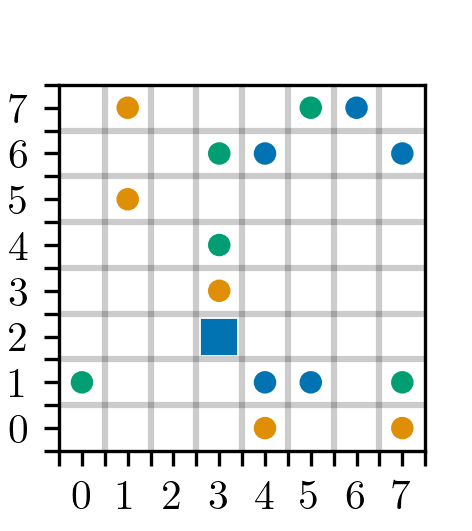
\includegraphics{"./figures/aux_1.png"}},
    s_{2,t} = \parbox[h][0.30\linewidth][c]{0.25\linewidth}{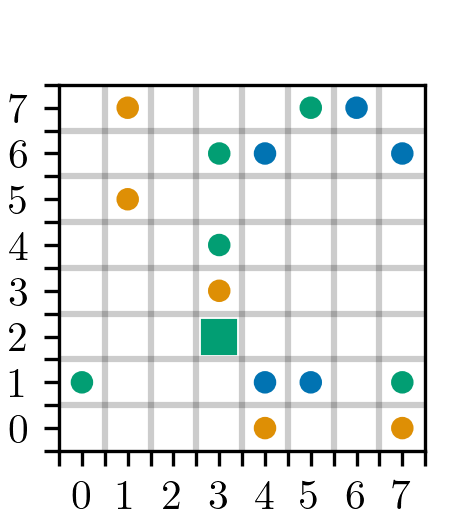
\includegraphics{"./figures/aux_2.png"}}$
\end{frame}

\begin{frame}{The manager approach}
  % \begin{algorithm}
With a trained manager, we use the following formula for the impact measurement:
\[ d(s_t,s_{t+1}) := \sum_{x=1}^2 \hat{V}_\phi(s_{x,t+1}) - \hat{V}_\phi(s_{x,t}).\]
  
\[ R^{\prime}(s_{t+1}) = R(s_{t+1}) + \lambda d(s_t,s_{t+1}).\]
\end{frame}

\begin{frame}{Training the manager}
  % \begin{algorithm}
  \begin{algorithmic}[1]
  \Require An MDP, a pre-trained policy $\pi$, and initial manager parameters $\phi_0$
  % \Ensure $y = x^n$
  \For{k = 0, 1, 2, \dots}
    \State Collect set of trajectories $\mathcal{D}_k = \{\tau_i\}$
    \State Randomly select augmentation $x$
    \State Fit manager estimate by regression using the mean-squared error:
    \[ \phi_{k+1} = \text{arg} \min_\phi \frac{1}{|\mathcal{D}_k|T} \sum_{\tau \in \mathcal{D}_k} \sum_{t=0}^T \left( \hat{V}_\phi(s^x_t) - V^\pi (s_t) \right)\]
  \EndFor
  \end{algorithmic}
  % \caption{Algorithm for training a manager network}
    % \label{alg:manager}
  % \end{algorithm}
\end{frame}

\begin{frame}{Experiments}
  The following environments will be used:
  \begin{table}
\footnotesize
\centering
    \begin{tabular}{l | c | c | c | c | c}
      environment & grid & observation & food objects & termination & max length\\ \hline
      MDP & $8 \times 8$ & - & 15 & 3 & 100\\
      POMDP & $8 \times 8$ & $5 \times 5$ & 15 & 3 & 100\\
      POMDP large & $16 \times 16$ & $5 \times 5$ & 30 & 6 & 200\\
    \end{tabular}
  \end{table}
  \begin{itemize}
    \visible<2->{\item Each with a stochastic and non-stochastic environment.}
    \visible<3->{\item Then evaluated using $\lambda \in \{0, 0.5, 1, 1.5, 2, 2.5, 3\}$}
  \end{itemize}
\end{frame}


\section{Results}

\begin{frame}{MDP}
  \centering
  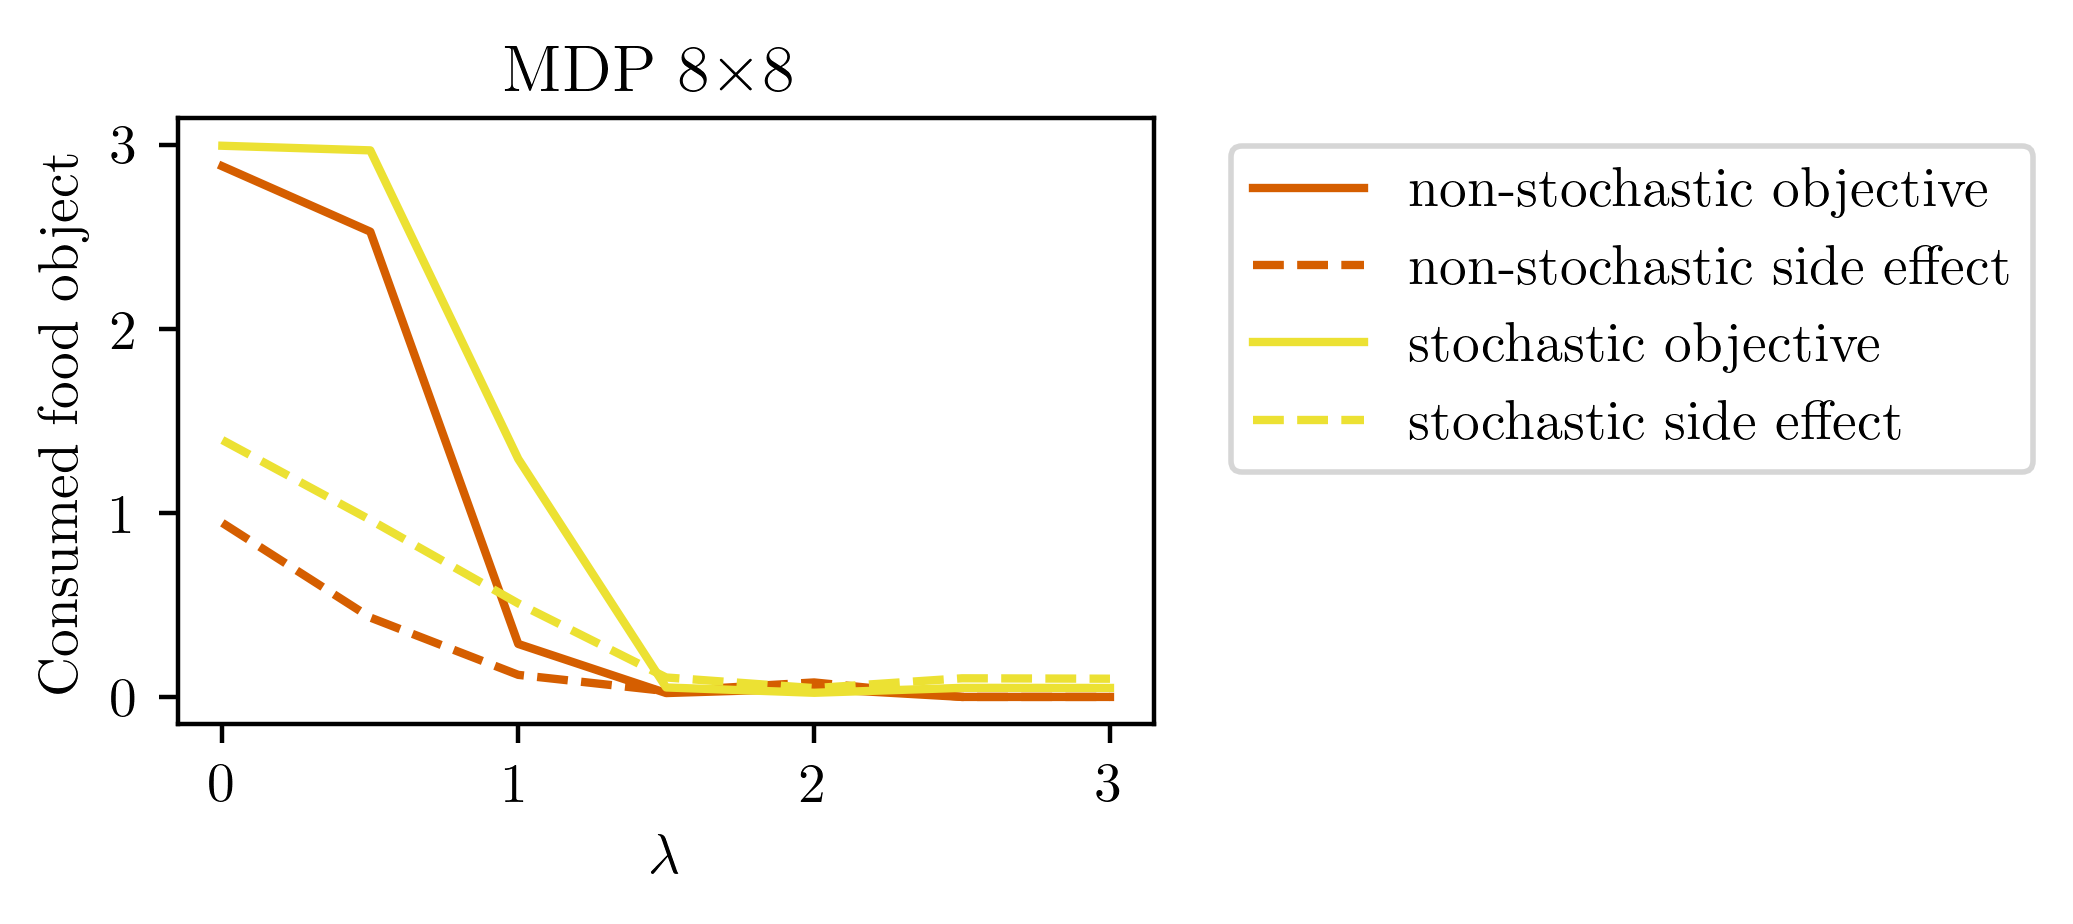
\includegraphics[scale=0.8]{"./figures/static_8x8_result_plot.png"}
\end{frame}

\begin{frame}{POMPD}
  \centering
  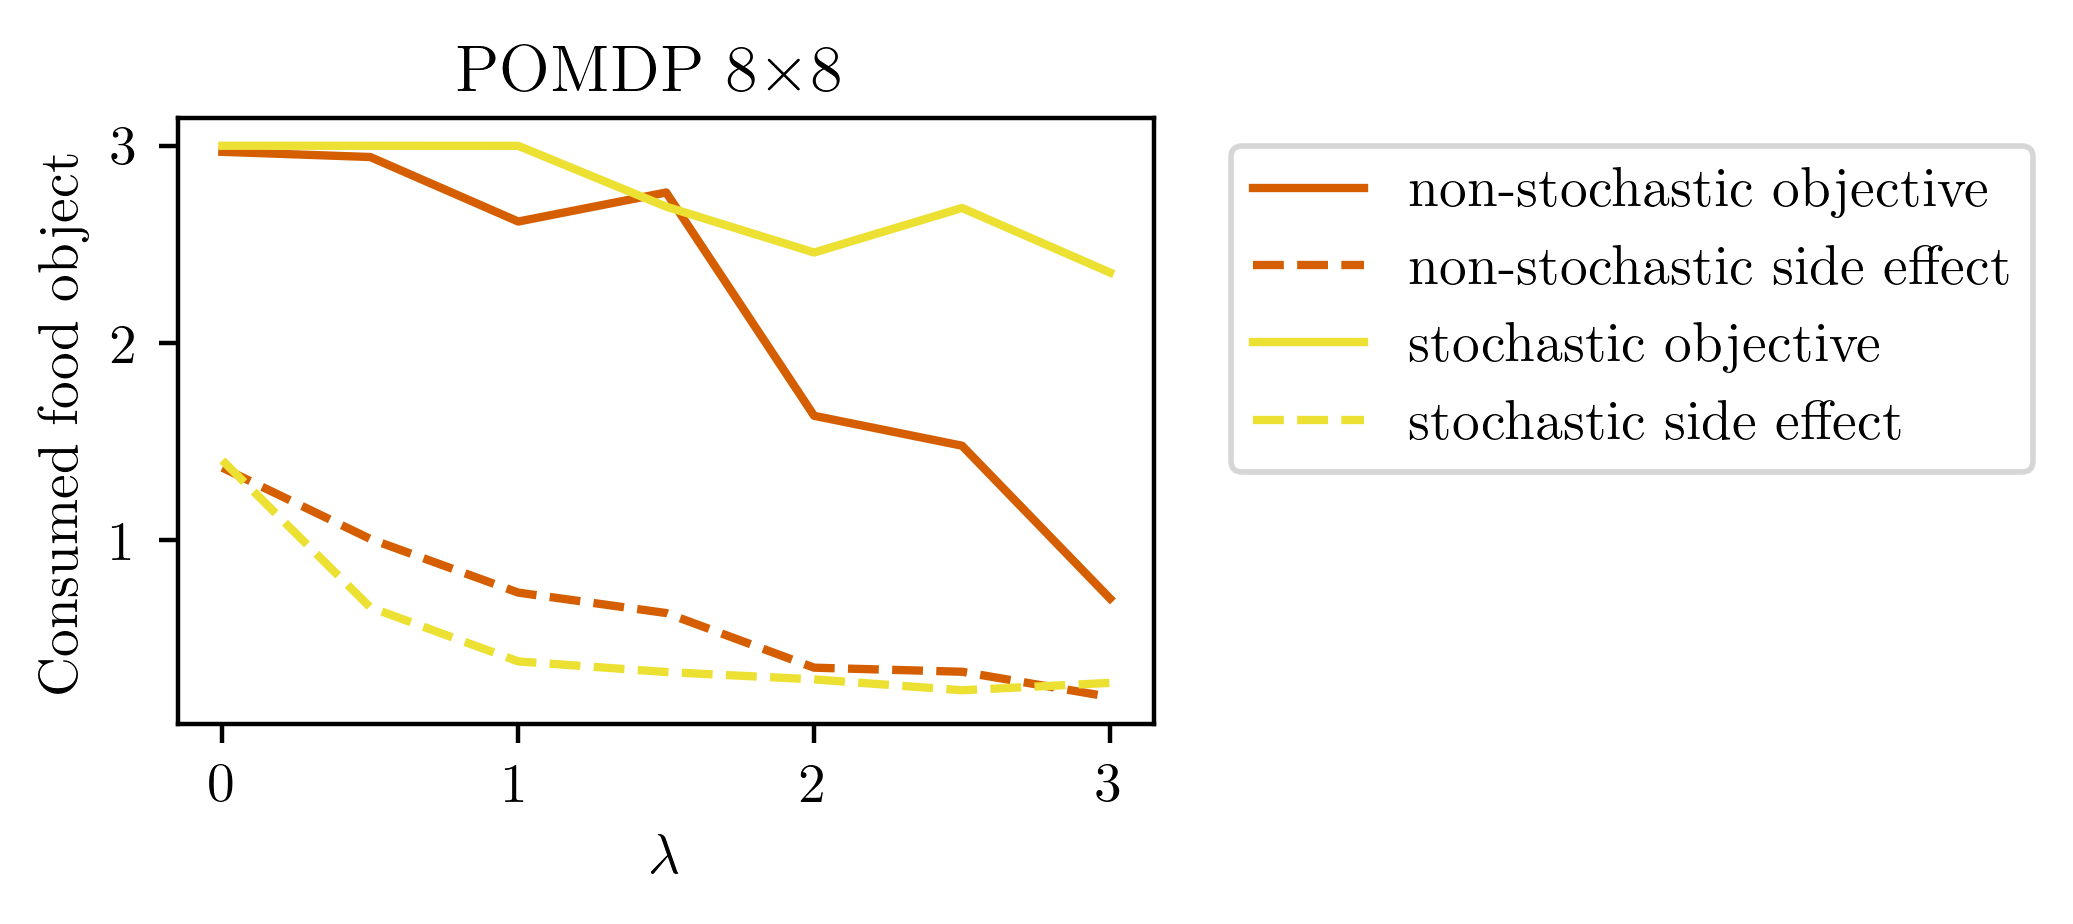
\includegraphics[scale=0.8]{"./figures/pomdp_8x8_result_plot.png"}
\end{frame}

\begin{frame}{POMDP large}
  \centering
  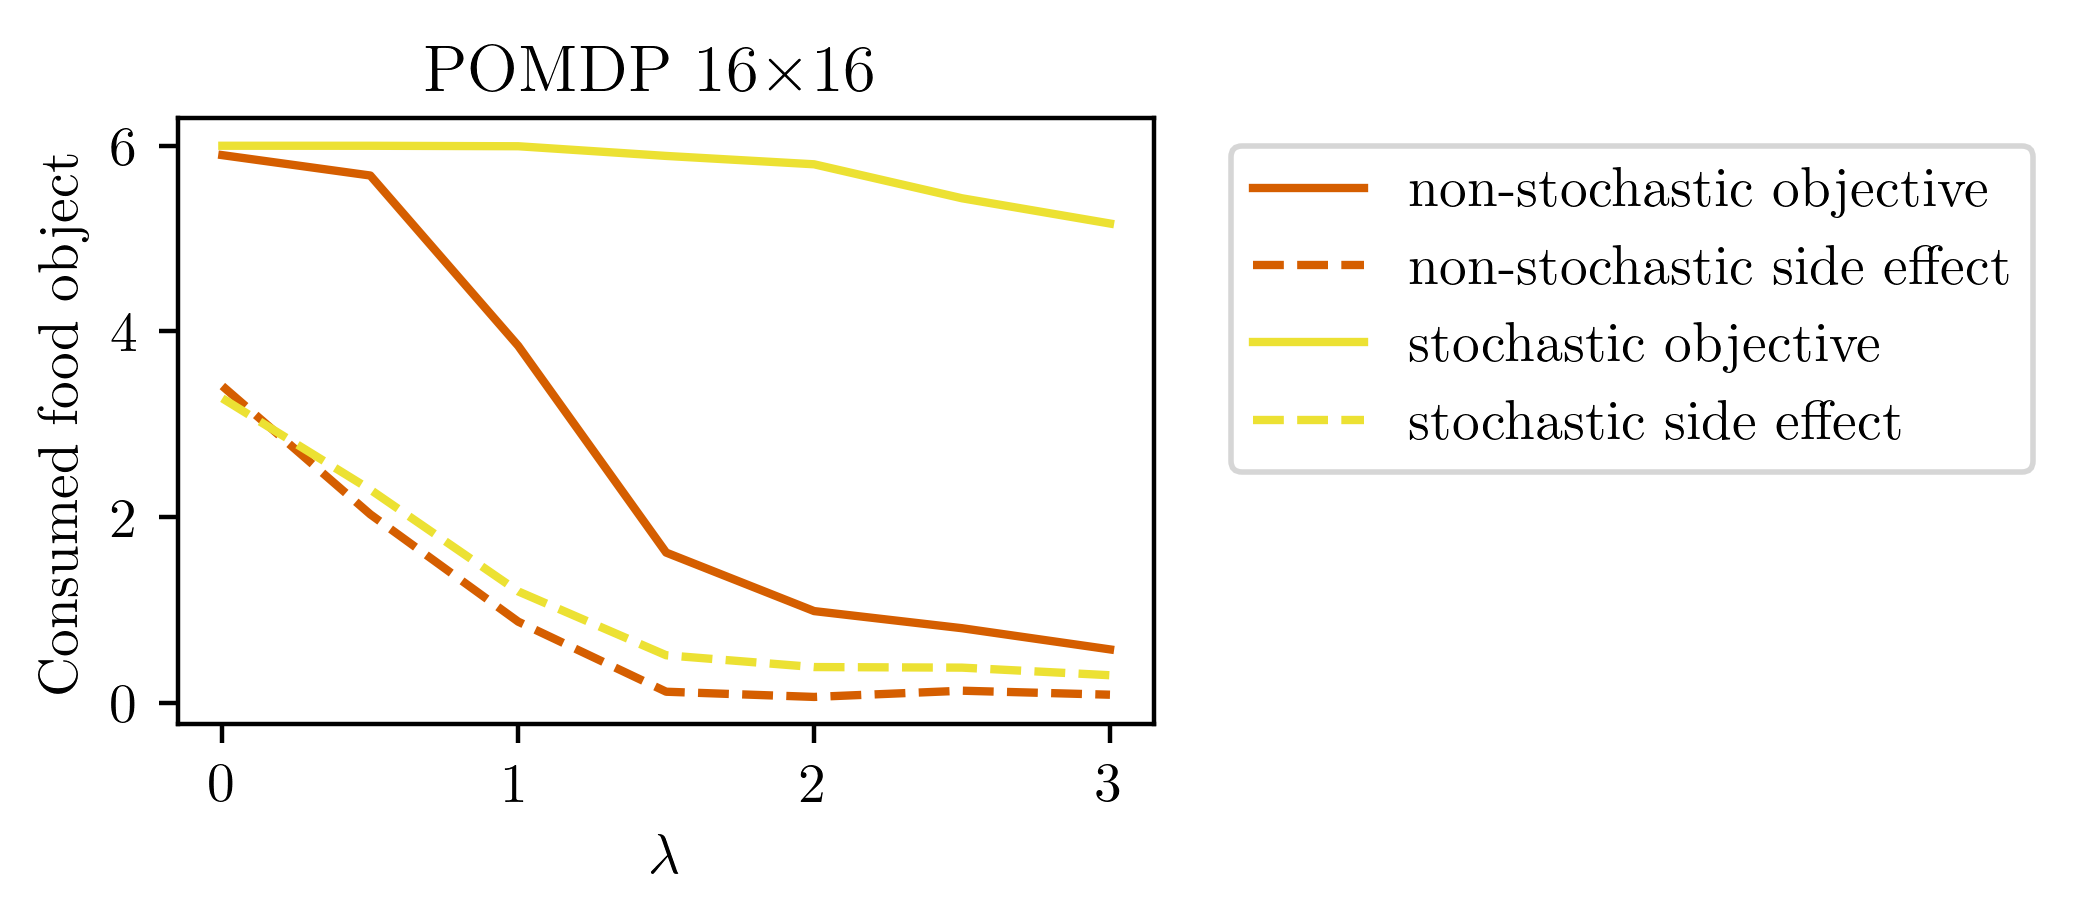
\includegraphics[scale=0.8]{"./figures/pomdp_16x16_result_plot.png"}
\end{frame}


\section{Conclusion}

\begin{frame}{Summary}
  \null
\end{frame}

\begin{frame}{End note}
  \null
\end{frame}

{\setbeamercolor{palette primary}{fg=black, bg=yellow}
\begin{frame}[standout]
  Questions?
\end{frame}
}

\bibliography{ref}
\bibliographystyle{apalike}

\end{document}
\begin{frame}{Artificial Intelligence}
  % A quick description of artificial intelligence, to make sure we are on the same page.

  On Wikipedias page about Arificial intelligence, we find the definition: 
  \onslide<2->{
    \begin{displayquote}
    Artificial Intelligence (AI) is intelligence demonstrated by\\ machines, as opposed to the natural intelligence displayed by animals including humans.
    \end{displayquote}}
  \onslide<3->{Olle Häggström in \textit{Tänkande Maskiner} clarification on intelligence:}
  \begin{itemize}
    \visible<4->{\item The quality that enables an entity to function effectively and with foresight in its environment.}
    \visible<5->{\item The ability to correctly perceive one's surrounding environment and act in a way that maximizes one's chances of achieving given goals.}
    % \item After that, I will explain the \textbf{manager approach}.
    % \item Finally, I will present the results.
  \end{itemize}
\end{frame}
\begin{frame}[fragile]{Metropolis}

  The \themename theme is a Beamer theme with minimal visual noise
  inspired by the \href{https://github.com/hsrmbeamertheme/hsrmbeamertheme}{\textsc{hsrm} Beamer
  Theme} by Benjamin Weiss.

  Enable the theme by loading

  \begin{verbatim}    \documentclass{beamer}
    \usetheme{metropolis}\end{verbatim}

  Note, that you have to have Mozilla's \emph{Fira Sans} font and XeTeX
  installed to enjoy this wonderful typography.
\end{frame}
\begin{frame}[fragile]{Sections}
  Sections group slides of the same topic

  \begin{verbatim}    \section{Elements}\end{verbatim}

  for which \themename provides a nice progress indicator \ldots
  
\end{frame}

\section{Titleformats}

\begin{frame}{Metropolis titleformats}
	\themename supports 4 different titleformats:
	\begin{itemize}
		\item Regular
		\item \textsc{Smallcaps}
		\item \textsc{allsmallcaps}
		\item ALLCAPS
	\end{itemize}
	They can either be set at once for every title type or individually.
\end{frame}

\subsection{Tricks}

{
    \metroset{titleformat frame=smallcaps}
\begin{frame}{Small caps}
	This frame uses the \texttt{smallcaps} titleformat.

	\begin{alertblock}{Potential Problems}
		Be aware, that not every font supports small caps. If for example you typeset your presentation with pdfTeX and the Computer Modern Sans Serif font, every text in smallcaps will be typeset with the Computer Modern Serif font instead.
	\end{alertblock}
\end{frame}
}

{
\metroset{titleformat frame=allsmallcaps}
\begin{frame}{All small caps}
	This frame uses the \texttt{allsmallcaps} titleformat.

	\begin{alertblock}{Potential problems}
		As this titleformat also uses smallcaps you face the same problems as with the \texttt{smallcaps} titleformat. Additionally this format can cause some other problems. Please refer to the documentation if you consider using it.

		As a rule of thumb: Just use it for plaintext-only titles.
	\end{alertblock}
\end{frame}
}

{
\metroset{titleformat frame=allcaps}
\begin{frame}{All caps}
	This frame uses the \texttt{allcaps} titleformat.

	\begin{alertblock}{Potential Problems}
		This titleformat is not as problematic as the \texttt{allsmallcaps} format, but basically suffers from the same deficiencies. So please have a look at the documentation if you want to use it.
	\end{alertblock}
\end{frame}
}

\section{Elements}

\begin{frame}[fragile]{Typography}
      \begin{verbatim}The theme provides sensible defaults to
\emph{emphasize} text, \alert{accent} parts
or show \textbf{bold} results.\end{verbatim}

  \begin{center}becomes\end{center}

  The theme provides sensible defaults to \emph{emphasize} text,
  \alert{accent} parts or show \textbf{bold} results.
\end{frame}

\begin{frame}{Font feature test}
  \begin{itemize}
    \item Regular
    \item \textit{Italic}
    \item \textsc{SmallCaps}
    \item \textbf{Bold}
    \item \textbf{\textit{Bold Italic}}
    \item \textbf{\textsc{Bold SmallCaps}}
    \item \texttt{Monospace}
    \item \texttt{\textit{Monospace Italic}}
    \item \texttt{\textbf{Monospace Bold}}
    \item \texttt{\textbf{\textit{Monospace Bold Italic}}}
  \end{itemize}
\end{frame}

\begin{frame}{Lists}
  \begin{columns}[T,onlytextwidth]
    \column{0.33\textwidth}
      Items
      \begin{itemize}
        \item Milk \item Eggs \item Potatos
      \end{itemize}

    \column{0.33\textwidth}
      Enumerations
      \begin{enumerate}
        \item First, \item Second and \item Last.
      \end{enumerate}

    \column{0.33\textwidth}
      Descriptions
      \begin{description}
        \item[PowerPoint] Meeh. \item[Beamer] Yeeeha.
      \end{description}
  \end{columns}
\end{frame}
\begin{frame}{Animation}
  \begin{itemize}[<+- | alert@+>]
    \item \alert<4>{This is\only<4>{ really} important}
    \item Now this
    \item And now this
  \end{itemize}
\end{frame}
\begin{frame}{Figures}
  \begin{figure}
    \newcounter{density}
    \setcounter{density}{20}
    \begin{tikzpicture}
      \def\couleur{alerted text.fg}
      \path[coordinate] (0,0)  coordinate(A)
                  ++( 90:5cm) coordinate(B)
                  ++(0:5cm) coordinate(C)
                  ++(-90:5cm) coordinate(D);
      \draw[fill=\couleur!\thedensity] (A) -- (B) -- (C) --(D) -- cycle;
      \foreach \x in {1,...,40}{%
          \pgfmathsetcounter{density}{\thedensity+20}
          \setcounter{density}{\thedensity}
          \path[coordinate] coordinate(X) at (A){};
          \path[coordinate] (A) -- (B) coordinate[pos=.10](A)
                              -- (C) coordinate[pos=.10](B)
                              -- (D) coordinate[pos=.10](C)
                              -- (X) coordinate[pos=.10](D);
          \draw[fill=\couleur!\thedensity] (A)--(B)--(C)-- (D) -- cycle;
      }
    \end{tikzpicture}
    \caption{Rotated square from
    \href{http://www.texample.net/tikz/examples/rotated-polygons/}{texample.net}.}
  \end{figure}
\end{frame}
\begin{frame}{Tables}
  \begin{table}
    \caption{Largest cities in the world (source: Wikipedia)}
    \begin{tabular}{lr}
      \toprule
      City & Population\\
      \midrule
      Mexico City & 20,116,842\\
      Shanghai & 19,210,000\\
      Peking & 15,796,450\\
      Istanbul & 14,160,467\\
      \bottomrule
    \end{tabular}
  \end{table}
\end{frame}
\begin{frame}{Blocks}
  Three different block environments are pre-defined and may be styled with an
  optional background color.

  \begin{columns}[T,onlytextwidth]
    \column{0.5\textwidth}
      \begin{block}{Default}
        Block content.
      \end{block}

      \begin{alertblock}{Alert}
        Block content.
      \end{alertblock}

      \begin{exampleblock}{Example}
        Block content.
      \end{exampleblock}

    \column{0.5\textwidth}

      \metroset{block=fill}

      \begin{block}{Default}
        Block content.
      \end{block}

      \begin{alertblock}{Alert}
        Block content.
      \end{alertblock}

      \begin{exampleblock}{Example}
        Block content.
      \end{exampleblock}

  \end{columns}
\end{frame}
\begin{frame}{Math}
  \begin{equation*}
    e = \lim_{n\to \infty} \left(1 + \frac{1}{n}\right)^n
  \end{equation*}
\end{frame}
\begin{frame}{Line plots}
  \begin{figure}
    \begin{tikzpicture}
      \begin{axis}[
        mlineplot,
        width=0.9\textwidth,
        height=6cm,
      ]

        \addplot {sin(deg(x))};
        \addplot+[samples=100] {sin(deg(2*x))};

      \end{axis}
    \end{tikzpicture}
  \end{figure}
\end{frame}
\begin{frame}{Bar charts}
  \begin{figure}
    \begin{tikzpicture}
      \begin{axis}[
        mbarplot,
        xlabel={Foo},
        ylabel={Bar},
        width=0.9\textwidth,
        height=6cm,
      ]

      \addplot plot coordinates {(1, 20) (2, 25) (3, 22.4) (4, 12.4)};
      \addplot plot coordinates {(1, 18) (2, 24) (3, 23.5) (4, 13.2)};
      \addplot plot coordinates {(1, 10) (2, 19) (3, 25) (4, 15.2)};

      \legend{lorem, ipsum, dolor}

      \end{axis}
    \end{tikzpicture}
  \end{figure}
\end{frame}
\begin{frame}{Quotes}
  \begin{quote}
    Veni, Vidi, Vici
  \end{quote}
\end{frame}

{%
\setbeamertemplate{frame footer}{My custom footer}
\begin{frame}[fragile]{Frame footer}
    \themename defines a custom beamer template to add a text to the footer. It can be set via
    \begin{verbatim}\setbeamertemplate{frame footer}{My custom footer}\end{verbatim}
\end{frame}
}

\begin{frame}{References}
  Some references to showcase [allowframebreaks] \cite{knuth92,ConcreteMath,Simpson,Er01,greenwade93}
\end{frame}

\section{Conclusion}

\begin{frame}{Summary}

  Get the source of this theme and the demo presentation from

  \begin{center}\url{github.com/matze/mtheme}\end{center}

  The theme \emph{itself} is licensed under a
  \href{http://creativecommons.org/licenses/by-sa/4.0/}{Creative Commons
  Attribution-ShareAlike 4.0 International License}.

  \begin{center}\ccbysa\end{center}

\end{frame}

{\setbeamercolor{palette primary}{fg=black, bg=yellow}
\begin{frame}[standout]
  Questions?
\end{frame}
}

\appendix

\begin{frame}[fragile]{Backup slides}
  Sometimes, it is useful to add slides at the end of your presentation to
  refer to during audience questions.

  The best way to do this is to include the \verb|appendixnumberbeamer|
  package in your preamble and call \verb|\appendix| before your backup slides.

  \themename will automatically turn off slide numbering and progress bars for
  slides in the appendix.
\end{frame}

\begin{frame}[allowframebreaks]{References}

  \bibliography{demo}
  \bibliographystyle{abbrv}

\end{frame}

\end{document}
